\chapter{IPFS}
\label{ipfs}

IPFS\footnote{\url{https://ipfs.io/}} stands for InterPlanetary File System and is a peer-to-peer distributed filesystem designed to make the Web faster, safer, and more open. In contrast with a standard filesystem, objects in IPFS are content-addressed by the cryptographic hash of their contents. In the case of the standard Web, when user wants some file, he needs to know on which server is a file located and the full path to the file (see figure \ref{webAddressing}). In IPFS user needs only to know the hash of the requested file. He does not care about the location of the file (see figure \ref{ipfsAddressing}). Let us take an MIT license text, and add it to IPFS.If somebody tries to add this license as a file to IPFS, it will return \texttt{QmWpvK4bYR7k9b1feM48fsk\-t2XsZfMaPfNnFxdbhJHw7QJ} every time. That is now and will be in the future, the \textit{content address} of that file. Later, when user try to get this file by its hash, he can get it from a random person that added it into IPFS in the past.

IPFS can easily represent a file system consisting of files and directories. A small file (less than 256 kB) is represented by an IPFS object with data being the file contents (plus a small header and footer). Note that the file name is not part of the IPFS object, so two files with different names and the same content will have the same IPFS object representation and hence the same hash. A large file (more than 256 kB) is represented by a list of links to file chunks that are less than 256 kB, and only minimal information specifying that this object represents a large file. Currently, there is no known size limitations uploaded file or directory. There are already some big datasets hosted on IPFS such as Geocities archive\footnote{\url{https://ipfs.io/ipfs/QmVCjhoEFC9vwvaa8bKyJgwAByP4MXSogcyDGoz4Lkc3ox}} (704TB) or Project Apollo Archives\footnote{\url{https://ipfs.io/ipfs/QmSnuWmxptJZdLJpKRarxBMS2Ju2oANVrgbr2xWbie9b2D}} (61GB).

IPFS provides API for manipulation with objects in several levels of abstraction. Two most used APIs are Files and Graph API. 
The files API\footnote{\url{https://github.com/ipfs/interface-js-ipfs-core/blob/master/SPEC/FILES.md}} enables users to use the File System abstraction of IPFS. Currently it has \texttt{add},  \texttt{cat},  \texttt{get} and  \texttt{ls} methods. In the future, there should be MFS (Mutable File System), that would add methods \texttt{chmod}, \texttt{cp}, \texttt{mv}, \texttt{rm}, \texttt{stat} and \texttt{touch}\footnote{\url{https://docs.ipfs.io/guides/concepts/mfs/}}.
Graph API\footnote{\url{https://github.com/ipfs/interface-js-ipfs-core/blob/master/SPEC/DAG.md}} is used in lower level of abstraction for manipulating with any IPFS object and creating links between objects. There are \texttt{put} and \texttt{get} methods available. 

\begin{figure}[h]
    \centering
    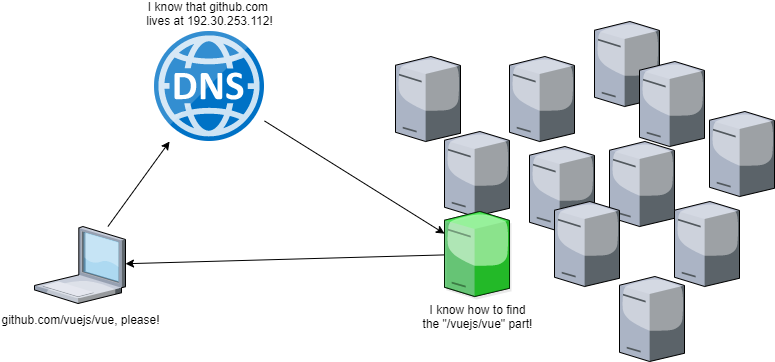
\includegraphics[width=11cm]{classicWebAddresing.png}
    \caption{Classic web addresing}
    \label{webAddressing}
\end{figure}

\begin{figure}[h]
    \centering
    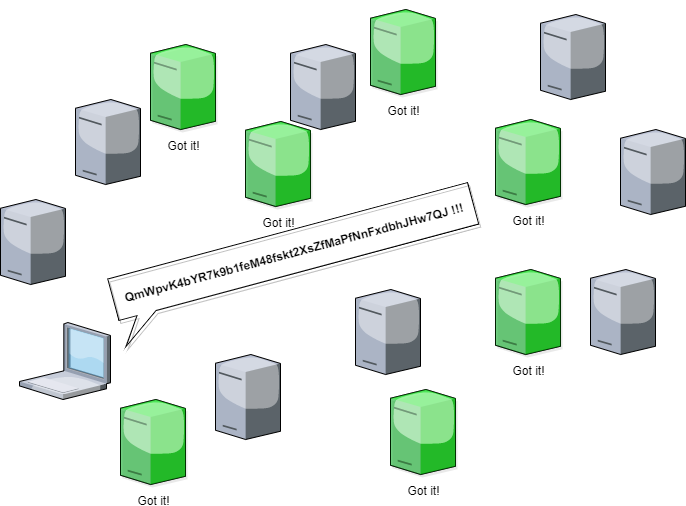
\includegraphics[width=11cm]{ipfsAddressing.png}
    \caption{Content-based addressing}
    \label{ipfsAddressing}
\end{figure}

\section{IPFS stack}
We can split IPFS into layers (see figure \ref{IPFSstack}). \textit{Libp2p}\footnote{\url{https://libp2p.io/}} is at the bottom, which is a peer-to-peer networking module, that handles peer and content discovery, transport, security, identity, peer routing, and messaging. \textit{IPLD} is the data model of the content-addressable web. It is providing linking between objects and multihash computing. On the top is \textit{IPFS} which allows to publish and share files (or any data).\cite{IPFSwhitepaper}


\begin{figure}[h]
    \centering
    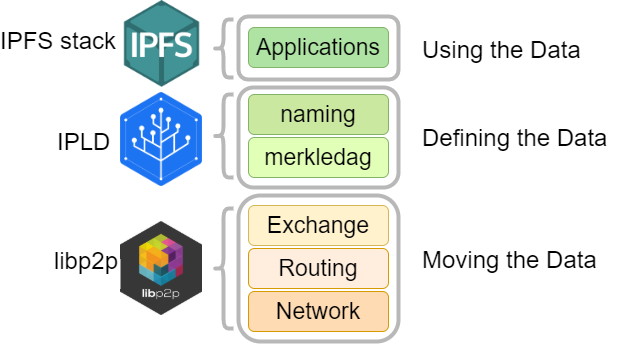
\includegraphics[width=11cm]{IPFSstack.png}
    \caption{IPFS stack}
    \label{IPFSstack}
\end{figure}


\section{libp2p}
Libp2p is a modular system of protocols, specifications and libraries that enable the development of peer-to-peer network applications. It provides NAT Traversal, Peer Discovery, Routing, Stream Multiplexing, Protocol Multiplexing, Encryption, Authentication and more. It grew out of IPFS to solve networking problems in p2p networks, but now it does not require or depend on IPFS. Today many projects use libp2p as their network transporting layer, which is responsible for the actual transmission and receipt of data from one peer to another. For both content discovery and peer routing, libp2p uses Kademlia-based distributed hash table. With Kademlia, libp2p iteratively routes requests closer to the desired peer or content using Kademlia routing algorithm\cite{kademlia}. In the future, Kademlia might be changed easily to some other solutions that implements a simple interface for publishing and requesting data and finding a peer.\cite{WebEngineering}


% \begin{figure}[h]
%     \centering
%     \begin{lstlisting}
%         // gets a particular peer's network address
%         FindPeer(node NodeId)

%         // stores a small metadata value in DHT
%         SetValue(key []bytes, value []bytes)

%         // retrieves small metadata value from DHT
%         GetValue(key []bytes)

%         // announces this node can serve a large value
%         ProvideValue(key Multihash)

%         // gets a number of peers serving a large value
%         FindValuePeers(key Multihash, min int)

%     \end{lstlisting}
%     \caption{libp2p interface}
%     \label{libp2pInterface}
% \end{figure}

\section{IPLD}
IPLD is providing linking and addressing objects with CID (Content ID). CID is hash-based self-describing content identifier (usually encoded to base58\footnote{\url{https://en.wikipedia.org/wiki/Base58}} format) which includes codec and multihash. Multihash is then further composed of hashtype and hash value. Let us look closer on the MIT license file, that we add to IPFS at the beginning of this chapter (see figure \ref{ipfs}). It's CID is \texttt{QmWpvK4bYR7k9b1feM48fsk\-t2XsZfMaPfNnFxdbhJHw7QJ}. It can be converted to human-readable format as can be seen in figure \ref{tab:CIDexample}, thanks to multicodec table\footnote{\url{https://github.com/multiformats/multicodec/blob/master/table.csv}}. We can see that this CID is encoded in base58 format and the file was stored using protobuf\footnote{\url{https://en.wikipedia.org/wiki/Protocol\_Buffers}} codec (this information is necessary to decode file correctly).



\begin{table}[]
    \centering
    \begin{tabular}{|ll|l|}
    \hline
    \textbf{Property}                  &             & \textbf{Value}                                                            \\ \hline
    Multibase                                        &             & base58btc                                                        \\ \hline
    Version                                          &             & cidv0                                                            \\ \hline
    Multicodec                                       &             & dag-pb                                                           \\ \hline
    \multicolumn{1}{|l|}{\multirow{3}{*}{Multihash}} & Hash Type   & sha2-256                                                         \\ \cline{2-3} 
    \multicolumn{1}{|l|}{}                           & Hash Length & 256                                                              \\ \cline{2-3} 
    \multicolumn{1}{|l|}{}                           & Hash        & 7e1b666c0327...3dc3022f \\ \hline
    \end{tabular}
    \caption{Example of human redable version of CID}
    \label{tab:CIDexample}
\end{table}

\section{IPFS}
IPFS is the top layer from the IPFS stack. It is used for pinning objects and files, naming system (see IPNS\footnote{\url{https://docs.ipfs.io/guides/concepts/ipns/}}) and keys management. File or object is automatically pinned when a user adds it (but other IPFS commands do not include automatic pinning). Pinning a CID tells an IPFS server that the data is important and must not be thrown away. When garbage collection is triggered on a node, any pinned content is automatically exempt from deletion. Non-pinned data may be deleted. The InterPlanetary Name System (IPNS) is a system for creating and updating mutable links to IPFS content. Since objects in IPFS are content addressed, an object address changes every time an object's content changes. A name in IPNS is the hash of a public key. It is associated with a record containing information about the hash it links to that is signed by the corresponding private key.

\section{IPNS}
Naming inside IPFS is governed by IPNS\footnote{\url{https://docs.ipfs.io/guides/concepts/ipns/}}, the InterPlanetary Naming System. IPNS takes ideas from SFS\footnote{\url{https://en.wikipedia.org/wiki/Self-certifying_File_System}} to enable the creation of cryptographically signed mutable pointers, which can be used to the creation of name records inside the network.

\section{Existing blockchain explorers in IPFS}
There are already stored a few blockchains of cryptocurrencies in IPFS. For browsing them we can use dedicated applications\footnote{\url{https://github.com/arcalinea/IPFS-Zcash-Explorer}} \footnote{\url{https://github.com/whyrusleeping/zcash-explorer}} or IPLD explorer\footnote{\url{https://explore.ipld.io/\#/explore/z43AaGEvwdfzjrCZ3Sq7DKxdDHrwoaPQDtqF4jfdkNEVTiqGVFW}}. Blockchains in IPFS are stored in raw binary format, so custom IPLD codec has to be created for every type of object. Using custom codecs for cryptocurrencies allows explorers to request blocks and transactions by its hash very fast, but there are also limitations.

\begin{itemize}
    \item Existing IPLD codecs for cryptocurrencies are very limited. Only a few of cryptocurrency codecs are currently available in IPLD (namely Leofcoin, Ethereum, Bitcoin, Zcash, Steller, Decred and Dash)\footnote{\url{https://github.com/multiformats/multicodec/blob/master/table.csv}}.
    \item Addresses are not stored in IPFS, because they are not part of a blockchain. This means the explorer needs to go through the entire blockchain for computing address balance or to find address transactions.
    \item No additional information (for example transaction value in US dollars) can be stored with objects because it would change content, and therefore hash of the object.
    \item There is no sorting or filtering. Explorer can only show the object (block or transaction) by its hash. 
\end{itemize}




% \begin{table}[]
% \centering
% \begin{tabular}{|l|l|l|}
% \hline
% \textbf{Name}        & \textbf{Code} & \textbf{Description}                             \\ \hline
% leofcoin-block       & 0x81          & Leofcoin Block                                   \\ \hline
% leofcoin-tx          & 0x82          & Leofcoin Transaction                             \\ \hline
% leofcoin-pr          & 0x83          & Leofcoin Peer Reputation                         \\ \hline
% eth-block            & 0x90          & Ethereum Block (RLP)                             \\ \hline
% eth-block            & 0x90          & Ethereum Block (RLP)                             \\ \hline
% eth-block-list       & 0x91          & Ethereum Block List (RLP)                        \\ \hline
% eth-tx-trie          & 0x92          & Ethereum Transaction Trie (Eth-Trie)             \\ \hline
% eth-tx               & 0x93          & Ethereum Transaction (RLP)                       \\ \hline
% eth-tx-receipt-trie  & 0x94          & Ethereum Transaction Receipt Trie (Eth-Trie)     \\ \hline
% eth-tx-receipt       & 0x95          & Ethereum Transaction Receipt (RLP)               \\ \hline
% eth-state-trie       & 0x96          & Ethereum State Trie (Eth-Secure-Trie)            \\ \hline
% eth-account-snapshot & 0x97          & Ethereum Account Snapshot (RLP)                  \\ \hline
% eth-storage-trie     & 0x98          & Ethereum Contract Storage Trie (Eth-Secure-Trie) \\ \hline
% bitcoin-block        & 0xb0          & Bitcoin Block                                    \\ \hline
% bitcoin-tx           & 0xb1          & Bitcoin Tx                                       \\ \hline
% zcash-block          & 0xc0          & Zcash Block                                      \\ \hline
% zcash-tx             & 0xc1          & Zcash Tx                                         \\ \hline
% stellar-block        & 0xd0          & Stellar Block                                    \\ \hline
% decred-block         & 0xe0          & Decred Block                                     \\ \hline
% dash-block           & 0xf0          & Dash Block                                       \\ \hline
% \end{tabular}
% \caption{Existing IPLD formats for cryptocurrencies}
% \label{ipldFormatsCrypto}
% \end{table}